\subsection{纤维方块投影的余均衡子}

设 X 与 Y 为拓扑空间，f 为从 X 到 Y 的一个连续映射。用 Z 表示纤维方块 \(X \times_{Y} X\)，用 \(p_{1}\) 与 \(p_{2}\) 表示从 Z 到 X 的两个投影。我们用 W 表示纤维积 \(X \times_{Y} X \times_{Y} X\)；对每个偶 \((s, t)\)（由 \(\{1,2,3\}\) 中的元素组成），用 \(q_{st}: W \to Z\) 表示由 \(q_{st}(x_{1}, x_{2}, x_{3}) = (x_{s}, x_{t})\) 定义的映射。

用 \(\operatorname{Coeg}(f)\) 表示群胚 \(\operatorname{Coeg}(\varpi(p_{1}),\varpi(p_{2}))\)，即两个态射 \(\varpi(p_{1})\)、\(\varpi(p_{2})\)（从庞加莱群胚 \(\varpi(Z)\) 到庞加莱群胚 \(\varpi(X)\)）的余均衡子。用 \(\gamma\colon\varpi(X)\to\operatorname{Coeg}(f)\) 表示规范的群胚态射。由于 \(f\circ p_{1}=f\circ p_{2}\)，群胚态射 \(\varpi(f)\circ\varpi(p_{1})\) 与 \(\varpi(f)\circ\varpi(p_{2})\)（从 \(\varpi(Z)\) 到 \(\varpi(Y)\)）相等；因此存在唯一的群胚态射 \(\varpi'(f)\colon\operatorname{Coeg}(f)\to\varpi(Y)\) 使得 \(\varpi'(f)\circ\gamma=\varpi(f)\)。

定义 1. --- 我们说映射 f 满足性质 (VK)，如果它是严格、满射的，并且态射 \(\varpi'(f)\) 是同构。

例 1. --- 在下列假设之一之下，此性质成立：

\begin{enumerate}
\def\labelenumi{(\roman{enumi})}
\item
  空间 X 与 Y 是可解圈的，空间 \(X \times_{Y} X\) 局部道路连通，映射 f 满射、逆紧、分离，且具有局部连通的纤维；
\item
  空间 X 与 Y 是可解圈的，映射 f 满射、逆紧、分离，且具有有限纤维，对角线 \(\Delta_{X}\) 在 \(X \times_{Y} X\) 中是开集且其补集局部连通；
\item
  空间 X 与 Y 是可解圈的，映射 f 满射、开，且具有道路提升性质；
\item
  Y 的每个点都有一个邻域，在该邻域之上存在映射 f 的连续截面。
\end{enumerate}

事实上，在这些假设的每一条之下，映射 \(f\) 都是满射；并且依据 I, 第~18~页，例 2，它也是严格的。最后，态射 \(\varpi'(f)\) 是同构：在假设 (i)、(ii) 或 (iii) 之下依据 IV, 第~398~页，定理 1，在假设 (iv) 之下依据（IV, 第~400~页，定理 2）。

II, 第~208~页的命题 5 描述了群胚 Coeg(f) 的迷向群。本节的目的在于：当 f 满足性质 (VK) 时，明显写出通过与群胚同构 \(\varpi'(f)\) 复合而由此得到的 Y 的庞加莱群的描述。随后的各号将用于讨论重要的特殊情形。

假设映射 f 满足性质 (VK)。

令 \(\mathsf{I} = \pi_0(\mathrm{X})\)，\(\mathsf{J} = \pi_0(\mathrm{Z})\)，\(\mathsf{K} = \pi_0(\mathrm{W})\)；对 \(j \in \mathsf{J}\) 与 \(s \in \{1,2\}\)，令 \(i_s(j) = \pi_0(p_s)(j)\)；对 \(k \in \mathsf{K}\) 与 \(s\)、\(t \in \{1,2,3\}\)，令 \(j_{st}(k) = \pi_0(q_{st})(k)\)。用 \(\Gamma\) 表示群胚态射偶 \((\varpi(p_1), \varpi(p_2))\)（从 \(\varpi(\mathrm{Z})\) 到 \(\varpi(\mathrm{X})\)）的框架（II, 第~185~页，定义 3）。它就是箭图 \((\mathsf{I}, \mathsf{J}, \pi_0(p_1), \pi_0(p_2))\)，因为拓扑空间的庞加莱群胚的轨道就是该空间的道路连通分支。

此外假设 Y 道路连通且非空。由 II, 第~200~页，注 2，\(\pi_0(\Gamma)\) 于是与群胚 Coeg(f) 的轨道集成双射；由于映射 \(f\) 满足性质 (VK)，群胚 Coeg(f) 同构于群胚 \(\varpi(Y)\)。于是图 \(\Gamma\) 连通且非空。

我们把 f 的范坎彭数据称为由下列元素组成的数据：

\begin{enumerate}
\def\labelenumi{(\roman{enumi})}
\item
  对每个 \(i \in \mathsf{I}\)，取 \(\mathsf{a}(i)\) 为道路连通分支 \(i\)（在 \(\mathbf{X}\) 中）的一点；
\item
  对每个 \(j \in J\)，取 Z 的道路连通分支 j 中的一点 \(\mathsf{b}(j) = (\mathsf{b}_{1}(j), \mathsf{b}_{2}(j))\)；
\item
  对每个 \(k \in \mathsf{K}\)，取 \(\mathsf{c}(k) = (\mathsf{c}_1(k), \mathsf{c}_2(k), \mathsf{c}_3(k))\) 为道路连通分支 \(k\)（在 \(\mathbf{W}\) 中）的一点；
\item
  对每个 \(j \in J\)，取 X 中一条道路的类 \(\beta_{1}(j)\)，该道路连接 \(\mathsf{b}_{1}(j)\) 与 \(\mathsf{a}(i_{1}(j))\)；再取 X 中一条道路的类 \(\beta_{2}(j)\)，该道路连接 \(\mathsf{b}_{2}(j)\) 与 \(\mathsf{a}(i_{2}(j))\)；
\item
  对每个 \(k \in K\) 与每个偶 \((s, t)\)（等于 \((1, 2)\)、\((2, 3)\) 或 \((1, 3)\)），取 Z 中一条道路的类 \(\gamma_{st}(k)\)，该道路连接 \((\mathsf{c}_{s}(k), \mathsf{c}_{t}(k))\) 与 \(\mathsf{b}(j_{st}(k))\)；
\item
  一个子箭图 \(\mathsf{T}\)（属于 \(\Gamma\)），其相伴图是图 \(\widetilde{\Gamma}\) 的极大树；
\item
  一个元素 \(i_{0}\)（属于 \(\mathsf{I}\)）。
\end{enumerate}

选取 \(f\) 的一个范坎彭数据。于是 \((\mathsf{a},\mathsf{b},\beta_{1},\beta_{2},\mathsf{T},i_{0})\) 是群胚态射偶 \((\varpi(p_{1}),\varpi(p_{2}))\)（从 \(\varpi(\mathrm{Z})\) 到 \(\varpi(\mathrm{X})\)）的基本配备（II, 第~192~页，定义 4）。此外，三元组

\[
\mathsf {z} = \left(\left(q _ {1 2} (\mathsf {c} (k)), 1\right), \left(q _ {2 3} (\mathsf {c} (k)), 1\right), \left(q _ {1 3} (\mathsf {c} (k)), - 1\right)\right)
\]

以及道路类 \((\gamma_{1,2}(k), \gamma_{2,3}(k), \gamma_{1,3}(k))\)（其中 k 取遍 K）定义了偶 \((\varpi(p_{1}), \varpi(p_{2}))\) 的一个补配备（II, 第~208~页，定义 3；II, 第~205~页，例；II, 第~205~页，注）。我们说如此定义的余均衡子 Coeg(f) 的完备配备是由我们所选取的 f 的范坎彭数据导出的。

对每个 \(j \in J\)，用 \(\varphi_{j} \colon \pi_{1}(Z, \mathsf{b}(j)) \to \pi_{1}(X, \mathsf{a}(i_{1}(j)))\) 与 \(\psi_{j} \colon \pi_{1}(Z, \mathsf{b}(j)) \to \pi_{1}(X, \mathsf{a}(i_{2}(j)))\) 表示由

\[
\varphi_ {j} = \operatorname{Int} (\beta_ {1} (j)) ^ {- 1} \circ (p _ {1}) _ {*}, \quad v \mapsto \beta_ {1} (j) ^ {- 1} ((p _ {1}) _ {*} (v)) \beta_ {1} (j)\tag{1}
\]

\[
\psi_ {j} = \mathrm{Int} (\beta_ {2} (j)) ^ {- 1} \circ (p _ {2}) _ {*}, \quad v \mapsto \beta_ {2} (j) ^ {- 1} ((p _ {2}) _ {*} (v)) \beta_ {2} (j),
\]

所定义的群同态，其中 \(v \in \pi_1(\mathbf{Z}, \mathfrak{b}(j))\)。对所有 \(k \in \mathsf{K}\) 与每个 \(s \in \{1,2,3\}\)，用 \(\lambda_s(k)\) 表示 X 中点 \(\mathfrak{a}(i_s(k))\) 处由下列式子定义的圈的类

\[
\lambda_ {1} (k) = \beta_ {1} (j _ {1 3} (k)) ^ {- 1} \cdot ((p _ {1}) _ {*} (\gamma_ {1 3} (k))) ^ {- 1} \cdot ((p _ {1}) _ {*} (\gamma_ {1 2} (k))) \cdot \beta_ {1} (j _ {1 2} (k)),\tag{2}
\]

\[
\lambda_ {2} (k) = \beta_ {2} (j _ {1 2} (k)) ^ {- 1} \cdot ((p _ {2}) _ {*} (\gamma_ {1 2} (k))) ^ {- 1} \cdot ((p _ {1}) _ {*} (\gamma_ {2 3} (k))) \cdot \beta_ {1} (j _ {2 3} (k)),
\]

\[
\lambda_ {3} (k) = \beta_ {2} (j _ {2 3} (k)) ^ {- 1} \cdot ((p _ {2}) _ {*} (\gamma_ {2 3} (k))) ^ {- 1} \cdot ((p _ {2}) _ {*} (\gamma_ {1 3} (k))) \cdot \beta_ {2} (j _ {1 3} (k)).
\]

用 \(\tau\) 表示从 Grp \((\Gamma)\) 到 \(\varpi(\mathrm{Y})\) 的唯一群胚态射，使得映射 Som \((\tau)\) 把 \(i \in \mathsf{I}\) 映为 \(f(\mathsf{a}(i))\)，且 Fl \((\tau)\) 把 \(j \in \mathsf{J}\) 映为道路 \(f_{*}(\beta_{1}(j))^{-1}f_{*}(\beta_{2}(j))\) 的类，该道路连接 \(f(\mathsf{a}(i_{1}(j)))\)

\pandocbounded{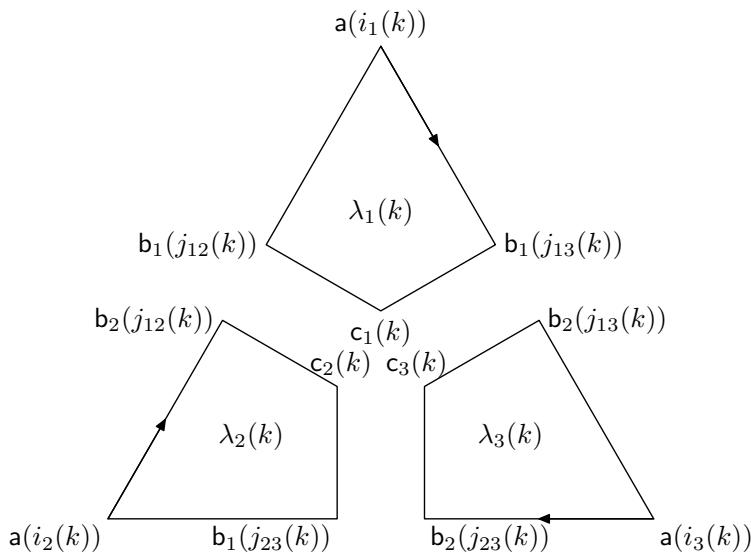
\includegraphics[keepaspectratio]{images/part003_b82e0de6.jpg}}

与 \(f(\mathsf{a}(i_2(j)))\)（在 Y 中）。对 \(i \in \mathsf{I}\)，令 \(d_i \in \mathrm{Grp}(\Gamma)\) 为连接 \(i_0\) 与 \(i\) 的唯一无折返道路（在树 \(\widetilde{\mathsf{T}}\) 中）的类，并令 \(\delta_i = \tau(d_i)\)。

回顾：若 S 是一个集合，则 F(S) 表示 S 上的自由群；在规范映射下元素 \(s \in S\) 在 F(S) 中的像记作 {[}s{]}，在不致混淆时甚至记作 s。

定理 1. --- 假设 Y 道路连通且 f 满足性质 (VK)。沿用前面的记号，存在唯一的群同态

\[
\mathsf {L} \colon \big (\underset {i \in \mathsf {I}} {\ast} \pi_ {1} (\mathrm{X}, \mathsf {a} (i)) \big) \ast \mathrm{F} (\mathrm{J}) \to \pi_ {1} (\mathrm{Y}, f (\mathsf {a} (i _ {0})))
\]

使得

\[
\begin{array}{l l} \mathsf {L} (v) = \delta_ {i} f _ {*} (v) \delta_ {i} ^ {- 1} & \text {for } i\in I \text { and } v\in\pi_{1} (X,a(i)), \\ \mathsf {L} (j) = \delta_ {i _ {1} (j)} \tau (j) \delta_ {i _ {2} (j)} ^ {- 1} & \text {for } j\in J. \end{array}
\]

此外，同态 L 是满射的，其核是包含下列元素的最小正规子群：

\[
\left(\mathrm{R} _ {1}\right) \quad \mathrm{r} _ {1} (j) = j \quad \text {for } j \text { in } \operatorname{Fl} (\mathsf {T});
\]

\[
\left(\mathrm{R} _ {2}\right) \quad \mathfrak {r} _ {2} (j, v) = \varphi_ {j} (v) j \psi_ {j} (v) ^ {- 1} j ^ {- 1} \quad \text {for } j \in \mathsf {J} \text { and } v \in \pi_ {1} (\mathrm{Z}, \mathfrak {b} (j));
\]

\[
\left(\mathrm{R} _ {3}\right) \quad \mathrm{r} _ {3} (k) = \lambda_ {1} (k) j _ {1 2} (k) \lambda_ {2} (k) j _ {2 3} (k) \lambda_ {3} (k) j _ {1 3} (k) ^ {- 1}, \quad \text {for } k \in \mathsf {K}.
\]

同态 L 的存在性与唯一性由自由积与自由群的泛性质得出。此外，这个同态是同态 \(\varpi'(f)_{\gamma(\mathsf{a}(i_0))}\)（由 \(\varpi'(f)\) 通过过渡到迷向群导出）与由 II, 第~208~页命题 5 所定义的群同态 \(\lambda\) 的复合，这里注意到所选取的范坎彭数据确定了群胚态射偶 \((\varpi(p_1), \varpi(p_2))\)（从 \(\varpi(\mathrm{Z})\) 到 \(\varpi(\mathrm{X})\)）的一个完备配备。由该命题，同态 \(\lambda\) 的像是群 \(\operatorname{Coeg}(f)_{\gamma(\mathsf{a}(i_0))}\)，其核是包含由关系 \((\mathrm{R}_1)\)、\((\mathrm{R}_2)\) 与 \((\mathrm{R}_3)\) 所定义的元素的最小正规子群。另一方面，由性质 (VK) 的定义，群胚态射 \(\varpi'(f)\) ： \(\operatorname{Coeg}(f) \to \varpi(\mathrm{Y})\) 是同构。定理于是得证。

